% Membrane and Ions
% Yotam Avital
\documentclass{article}
\usepackage{tikz}
\begin{document}
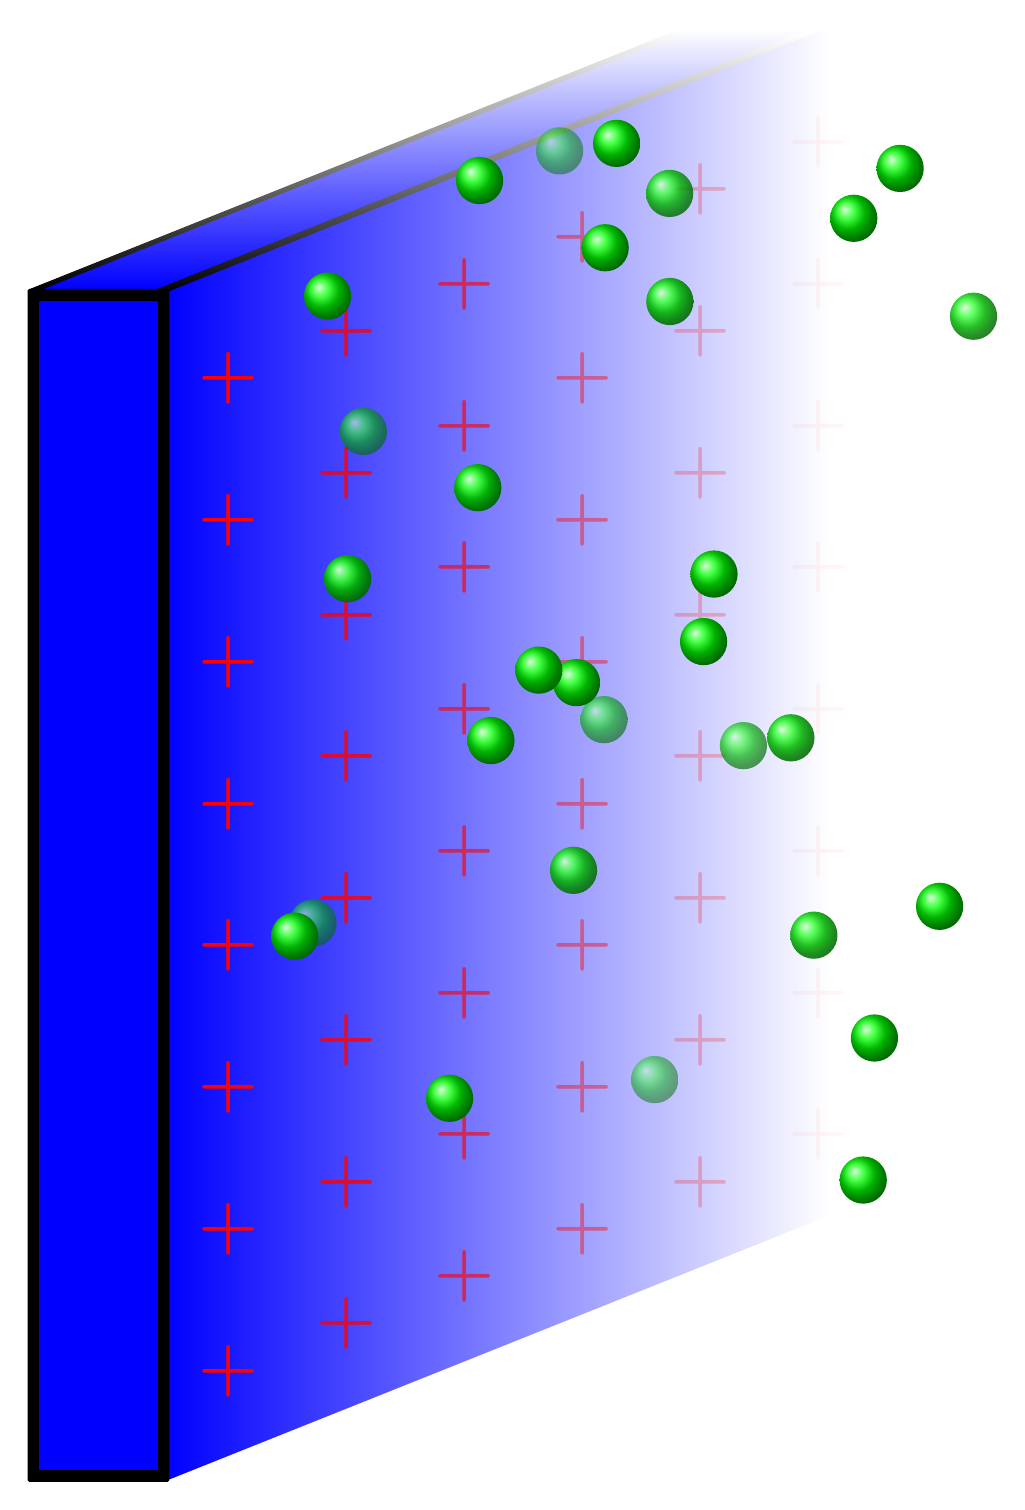
\begin{tikzpicture}[x=3cm, y=3cm]
\begin{scope}[every node/.append style={
      yslant=0,xslant=0},yslant=0,xslant=2.5
  ]
  \shade[bottom color = black, top color = white] (-12.54, 5)
    rectangle +(0.1, 1.1);
  \shade[bottom color = blue, top color = white] (-12.48,5)
    rectangle +(0.5,1.1);
  \shade[bottom color = black, top color = white] (-12, 4.98)
    rectangle +(0.1, 1.1);
\end{scope}

\begin{scope}[every node/.append style={
      yslant=0,xslant=0},yslant=0.4,xslant=0
  ]
  \shade[left color = blue, right color = white, rounded corners=1]
    (0.54,-0.26) rectangle +(2.8,5.03);
  \foreach \x in {0.8,1.3,...,3.3}{
    \foreach \y in {0.1, 0.7,..., 4.8}{
      \pgfmathsetmacro{\val}{1-(\x-0.8)/2.6}
      \node [color = red, opacity =\val] at (\x ,\y) {\Huge{\textbf +}};
    }
  }
\end{scope}

\pgfmathsetseed{10}

  \foreach \i in {1,2,...,30}{
%    \pgfmathsetmacro{\x}{(rand*0.5 + 1)*4 + 1}
%    \pgfmathsetmacro{\y}{(rand*0.5 + 1)*3.9 + 2 }
    \pgfmathsetmacro{\x}{(rand*0.5 + 1)*3 - 0.5}
    \pgfmathsetmacro{\y}{(rand*0.5 + 1)*4.7-1.2}
    %    \pgfmathsetmacro{\opacVal}{0.95*(\x-2.5)/4 + rand*0.05}
    \pgfmathsetmacro{\opacVal}{rand*0.5+1}
    \shade [ball color = green, opacity = \opacVal] (\x,\y) circle (0.1);
  }

\fill [fill = black,rounded corners= 0.6] (-0.05,-0.05)
  rectangle +(0.6,5.05);
\fill [fill = blue] (0,0) rectangle +(0.5,4.95);
\end{tikzpicture}
\end{document}
